\documentclass{beamer}
%\usetheme{Madrid} % My favorite!
%\usetheme{Boadilla} % Pretty neat, soft color.
\usetheme{default}
%\usetheme{Warsaw}
%\usetheme{Bergen} % This template has nagivation on the left
%\usetheme{Frankfurt} % Similar to the default
%with an extra region at the top.
%\usecolortheme{seahorse} % Simple and clean template
%\usetheme{Darmstadt} % not so good
% Uncomment the following line if you want %
% page numbers and using Warsaw theme%
%\setbeamertemplate{footline}[page number]
%\setbeamercovered{transparent}
%\setbeamercovered{invisible}
% To remove the navigation symbols from
% the bottom of slides%
\setbeamertemplate{navigation symbols}{}
%
%\usepackage{fullpages}
%\usepackage{psfig}
\usepackage{epstopdf}

%\usepackage{subfig}
%\usepackage{tikz}
%\usepackage{chronology}


\usepackage{amsmath}    % need for subequations
\usepackage{verbatim}   % useful for program listings
\usepackage{color}      % use if color is used in text
\usepackage{subfigure}  % use for side-by-side figures
\usepackage{hyperref}   % use for hypertext links, including those to external documents and URLs
\usepackage{amssymb,latexsym, amsmath}
\usepackage{graphicx}
\usepackage{amsthm}
\usepackage{multirow}
\usepackage{float}
%\usepackage{subcaption}
\usepackage{caption}
%\usepackage{subcaption}
%\usepackage{bm} % For typesetting bold math (not \mathbold)
%\logo{\includegraphics[height=0.6cm]{yourlogo.eps}}
\theoremstyle{Definition}
\newtheorem{defi}{Definition}
\newtheorem{propo}{Proposition}
%\graphicspath{{graphs//}}

\title{Risk Aversion or Mistaken  Beliefs?\footnote{Alternative title: ``Three Martingales and More''}
} % \\
      % Alternative Likelihood Ratios} %\\
       %Many Martingales}
\author{Thomas J. Sargent }
\date{March 2026\ {\small  New York University}}
% \today will show current date.
% Alternatively, you can specify a date.
%

%----------------------------------------------------------------------------------------------
\begin{document}
\begin{frame}
\titlepage
\end{frame}



\begin{frame}{Risks and beliefs}


 \begin{align*}
         \varepsilon & \cr
         \phi(\varepsilon) & \propto \exp\left(- \frac{1}{2} \varepsilon' \varepsilon\right) \sim {\mathcal N}(0,I) \cr
         m(\varepsilon) &  = \exp \left( -\lambda' \varepsilon - \frac{1}{2} \lambda' \lambda \right) \geq 0  \Rightarrow 
     E m(\varepsilon)  = 1 \cr
    \hat \phi(\varepsilon)  & =  m(\varepsilon) \phi(\varepsilon)  \propto \exp\left( - \frac{1}{2} (\varepsilon - \lambda)'(\varepsilon - \lambda)\right)  \sim {\mathcal N}(-\lambda, I) \cr
               \textrm{entropy} & \equiv  E m(\varepsilon) \log m (\varepsilon) = \frac{1}{2} \lambda'\lambda
        \end{align*}
%
%\bigskip
%\footnotesize{ $$\textrm{entropy} = \frac{1}{2} \lambda'\lambda $$    }

%
% \medskip
% \noindent
%  $$ \hat \phi(\varepsilon) = m(\varepsilon) \phi(\varepsilon) $$
\end{frame}



\begin{frame}{Risks and beliefs}


 \begin{align*}
         \varepsilon & \sim \quad {\color{red}{\textrm{ risks to be taken and priced}}} \cr
         \phi(\varepsilon) & \propto \exp\left(- \frac{1}{2} \varepsilon' \varepsilon\right) \sim {\mathcal N}(0,I) , \quad  {\color{red}{\textrm {a probability density}}} \cr
         m(\varepsilon) &  = \exp \left( -\lambda' \varepsilon - \frac{1}{2} \lambda' \lambda \right) \geq 0  \Rightarrow 
     E m(\varepsilon)  = 1 , \cr
      &  {\color{red}{\textrm {a likelihood ratio}}}  \cr
    \hat \phi(\varepsilon)  & =  m(\varepsilon) \phi(\varepsilon)  \propto \exp\left( - \frac{1}{2} (\varepsilon - \lambda)'(\varepsilon - \lambda)\right)  \sim {\mathcal N}(-\lambda, I) , \cr
    &  {\color{red}{\textrm {a twisted probability density}}}  \cr
               \textrm{entropy} & \equiv  E m(\varepsilon) \log m (\varepsilon) = \frac{1}{2} \lambda'\lambda
        \end{align*}
%
%\bigskip
%\footnotesize{ $$\textrm{entropy} = \frac{1}{2} \lambda'\lambda $$    }

%
% \medskip
% \noindent
%  $$ \hat \phi(\varepsilon) = m(\varepsilon) \phi(\varepsilon) $$
\end{frame}

\begin{frame}{Likelihood ratios (multiplicative martingale increments)}
\begin{table}
\begin{center}
\begin{tabular}{lll}
Probability  & Likelihood ratio & Describes \\ %$m_{t+1}$ \\
\hline\\
econometric  &  1 &  macro risk factors \\
         &  &   \\
risk neutral  & $m_{t+1}^\lambda $ & prices of risks  \\
         & &   \\
mistaken &  $m_{t+1}^w $  & experts'  forecasts  \\
         & &   \\
doubtful & $m_{t+1} \in {\mathcal M} $ & misspecification fears  \\
          & & \\
%\hline \\
\end{tabular}
\caption*{ $m_{t+1}^b = \exp\left(-b_t' \varepsilon_{t+1} - \frac{b_t' b_t}{2} \right) $;  $b_t= 0$ or $\lambda_t$ or $w_t$ or $\ldots$}
\end{center}
\end{table}

\end{frame}





\begin{frame}{Risks,  Returns, Mistakes}

 Effects of {\em risk aversion} and {\em wrong beliefs} are confounded

\begin{itemize}

\item Rational expectations and risk aversion: 
\begin{itemize}
\item Higher mean returns compensate for higher risks (variances)   
\end{itemize}
\item Representative investor with wrong beliefs:
\begin{itemize}
 \item observed average returns depend on \textcolor{red}{both}  risk aversion \textcolor{red}{and}   misunderstood returns distribution
 \end{itemize}
\end{itemize}

\end{frame}



\begin{frame}{Risks,  Returns, Mistakes}


\begin{itemize}
\item Wrong beliefs contribute {\em ``stochastic discount factor shocks''} 
\item Can ``misunderstandings'' explain observed countercyclical risk prices?
\end{itemize}

\end{frame}

%
%\begin{frame}{Young researchers}
% \begin{itemize}
%  \item Jaroslav Borovi\v{c}ka
%  \item Anmol Bhandari
%  \item Timothy Christensen
%  \item B\'{a}lint Sz\H{o}ke\
%   \end{itemize}
%
%
%
%\end{frame}
%
%
%\begin{frame}{Middle aged researchers}
% \begin{itemize}
% \item Monika Piazzesi
% \item Jessica Wachter
%  \item Amir Yaron
%  \item Stanley Zin
%  \item Lars Hansen
% \end{itemize}
%
%
%
%\end{frame}


\begin{frame}{1970's-1980's Informal Justification of Rational Expectations}


Outcome of learning from an infinite history:\\
least squares learning converges to rational expectations

 \begin{itemize}
    \item Agents know  correct functional forms
  \item Proof technique: stochastic approximation --  partition  dynamics into fast  (justifying a  LLN) and slow (justifying an ODE)
  \item Long intertemporal dependencies make  {\textcolor{red}{rates of convergence  slow}}
 \end{itemize}

\end{frame}


\begin{frame}{Good econometricians}

\begin{itemize}
\item Have  limited data and  only  hunches about functional forms
\item Fear that their fitted   models are incorrect
%\item Respect Oliver Cromwell's rule: ``think it possible that you might be mistaken''
\end{itemize}

\end{frame}

\begin{frame}{An agent who is  like a good econometrician}
\begin{itemize}
\item Has parametric model estimated from limited  data
\item Acknowledges that many other  specifications fit  nearly as well
\begin{itemize}
\item Other parameter values
 \item Other functional forms and omitted variables
 \begin{itemize}
  \item Neglected nonlinearities and  history dependencies
  \end{itemize}
\end{itemize}
\item Fears that one of those other models actually prevails
\item Seeks ``good enough'' decisions under \textcolor{red}{all} such alternative models (``robustness'')
\end{itemize}
\end{frame}



\begin{frame}{Econometrician's and agent's shared model}

%\textbf{Baseline dynamics:}

\begin{eqnarray*}
x_{t+1} & = & A x_t + C \varepsilon_{t+1} \cr
y_{t+1} & = & D x_t + G \varepsilon_{t+1} \cr
\varepsilon_{t+1} & \sim &{\mathcal N}(0,I) \cr
r_t & = & \bar r x_t \cr
d_t & = & \bar d x_t
\end{eqnarray*}

$y_{t+1}$: utility-relevant variables

$r_t$: risk-free one-period interest rate

$d_t$: payout process from an asset

\end{frame}

\begin{frame}{Want}

Price at $t$ of a claim to  random payout stream $\{d_{t+j}\}_{j=1}^\infty$


\end{frame}

\begin{frame}{Get}

\begin{itemize}
\item A sequence of models distinguished by beliefs
\item Stochastic discount factor shocks
\item Convenient mathematical forms
\item Secret weapon: likelihood ratio
\end{itemize}

\end{frame}



\begin{frame}{Rational expectations with risk neutral representative investor}
\textbf{Stock prices} (Shiller):

Stock price $p_t$:

\begin{eqnarray*}
p_t & =  & \exp(-r_t) E_t (p_{t+1} + d_{t+1}) \cr
\end{eqnarray*}


\textbf{Expectations theory of term structure of interest rates} (Hicks-Shiller):
time $t$ price $p_t(n)$ of a zero coupon   risk-free claim to one dollar at time $t+n$

\begin{eqnarray*}
p_t(1) &= &\exp(- r_t) \cr
p_t(n+1) & = & \exp(-r_t) E_t p_{t+1}(n)  \Rightarrow \cr
p_t(n) & = & \exp(B_n x_t)
\end{eqnarray*}

\end{frame}



\begin{frame}{Rational expectations with risk neutral representative investor}
Works
\begin{itemize}
\item ``Pretty well'' for conditional means
\item Less well for  conditional variances (Shiller ``volatility puzzles'')
\end{itemize}
\end{frame}

\begin{frame}{Wouldn't it  be nice  $\ldots$}



$\ldots$ if we could make versions of the  same formulas work even when investors
\begin{itemize}
\item Are risk averse
\item Don't have rational expectations
\end{itemize}



\medskip

``Ask and it shall be given'' (if you don't ask  too much)

\end{frame}


\begin{frame}{Key tool: likelihood ratio}
Let
\begin{eqnarray*}
 m_{t+1}^\lambda & = & \exp\left(-\lambda_t \varepsilon_{t+1} - \frac{1}{2} \lambda_t ' \lambda_t \right) \cr
 \lambda_t &= &  \lambda x_t \cr
 E_t m_{t+1}^\lambda &= &1, \quad m_{t+1}^\lambda \geq 0
 \end{eqnarray*}


\begin{itemize}
%\item Note:
%\[ E_t m_{t+1} = 1, \quad m_{t+1} \geq 0 \]
\item  $m_{t+1}^\lambda$ is  a likelihood ratio that distorts  conditional distribution of $\varepsilon_{t+1}$.
\item Multiplication of ${\mathcal N}(0, I)$  by $m_{t+1}^\lambda$ shifts  density of
$\varepsilon_{t+1}$ to ${\mathcal N}(- \lambda x_t, I)$.
\item Covariances of returns with $m_{t+1}^\lambda$ affect   mean returns
\begin{itemize}
\item Risk aversion
\item Apparent ``misunderstandings''
\end{itemize}
\end{itemize}
\end{frame}


\begin{frame}{Likelihood ratio application number 1}

\begin{itemize}
\item  Likelihood ratio expresses risk aversion
\item $\lambda_t$ is price  representative agent charges for bearing exposure to $\varepsilon_{t+1}$
\item Expected return of an asset depends on how its payout covaries with  $\varepsilon_{t+1}$

\end{itemize}
\end{frame}



\begin{frame}{Modern (post Shiller) asset pricing}


\textbf{Stock price} (Lucas-Hansen):
\begin{eqnarray*}
p_t & =  &\exp(-r_t) E_t ({\color{red} m_{t+1}^\lambda} (p_{t+1} + d_{t+1})) \cr
\end{eqnarray*}


\textbf{Term structure} (Dai-Singleton-Backus-Zin):

\begin{eqnarray*}
p_t(1) &= &\exp(- r_t) \cr
p_t(n+1) & = & \exp(-r_t) E_t ({\color{red} m_{t+1}^\lambda} p_{t+1}(n)) \cr
p_t(n) & = & \exp(B_n x_t)
\end{eqnarray*}

``Ask and it shall be given'' works (this time)
\end{frame}


\begin{frame}{``Risk-neutral'' dynamics}





\begin{eqnarray*}
x_{t+1}  & = & (A - {\color{red} C  \lambda}) x_t + C \tilde \varepsilon_{t+1} \cr
\tilde \varepsilon_{t+1} & \sim & {\mathcal N}(0,I) \cr
\lambda_t & = & \lambda x_t
\end{eqnarray*}

\end{frame}

\begin{frame}{Risk-neutral  dynamics}


\begin{itemize}
\item
Risk neutral dynamics assert that  shock distribution $\varepsilon_{t+1}$
has conditional mean $ - \lambda_t  $
instead of
$ 0 $.
\item Dependence of $\lambda_t = \lambda x_t $ on  $x_t$ modifies dynamics relative to  econometrician's  model
\end{itemize}

\end{frame}


\begin{frame}{Mathematical expectation under twisted distribution}

Mathematical expectation  of  $y_{t+1}$ under probability distribution twisted by likelihood ratio $m_{t+1}$
is

$$ \tilde E_t y_{t+1} = E_t m_{t+1} y_{t+1}$$

%\begin{itemize}
%\item LHS: a mean
%\item RHS: a covariance
%\end{itemize}

\end{frame}

\begin{frame}{Risk-neutral pricing represented}

With respect to risk neutral dynamics, modern (Backus-Zin) term structure theory
is


\begin{eqnarray*}
p_t(1) &= &\exp(- r_t) \cr
p_t(n+1) & = & \exp(-r_t) \tilde E_t ( p_{t+1}(n)) \Rightarrow \cr
p_t(n) & = & \exp(\tilde B_n x_t)
\end{eqnarray*}

where $\tilde E_t$ is an expectation with respect to the risk-neutral  measure.

\begin{itemize}
\item Same formulas as (Shiller) rational expectations asset pricing theory, but $\ldots$
 \item Take mathematical expectations with respect to a   probability measure \color{red}{twisted by risk-aversion}
\end{itemize}
\end{frame}

%
%
%\begin{frame}{Term structure (Backus-Zin)}
%
%\begin{eqnarray*}
%p_t(1) &= &\exp(- r_t) \cr
%p_t(n+1) & = & \exp(- r_t) \tilde E_t ( p_{t+1}(n)) \cr
%p_t(n) & = & B_n x_t
%\end{eqnarray*}
%
%where $ \tilde E_t$ is mathematical expectation with respect to twisted (aka risk-neutral)  model
%
%\end{frame}



\begin{frame}{Likelihood ratio number 2,  $m_{t+1}^w$}

Mistaken beliefs (according to the econometrician's model)

\bigskip
\bigskip

Relative to model of risk-averse representative investor with rational expectations, model of
risk-neutral  investor with mistaken beliefs has 

\begin{itemize}
%\item Risk aversion
%\item Mistaken beliefs (according to the econometrician's model) %Probability distortion (twisted dynamics)
\item Identical asset pricing formulas  %\textbf{These are observationally equivalent}
\item Identical econometric fits 
\end{itemize}


Insight of Hansen, Sargent, Tallarini (1999) and  Piazzesi, Salomao, Schneider (2015)

\end{frame}
\begin{frame}{Identification challenge}
$\lambda_t$ can be interpreted as either

\begin{itemize}
\item Risk price vector expressing ``representative'' agent's risk aversion, or
\item Representative agent's belief distortion relative to econometrician's model
\end{itemize}

To distinguish, need more information  (Piazzesi, Salomao, Schneider, PSS) or more theory (Hansen and Sz\H{o}ke) or both (Sz\H{o}ke)

\end{frame}



\begin{frame}{More information: experts' forecasts are biased}
Piazzesi, Salomao, Schneider (2015)

\begin{itemize}
\item Representative agent's risk aversion leads him to price risks $\varepsilon_{t+1}$ with prices $\lambda_t^* = \lambda^* x_t$
\item Representative agent has twisted beliefs $(A^*, C) = (A- C w^*, C)$  relative to econometrician's model $(A,C)$
\item Professional forecasters use  twisted beliefs $(A^*,C) $ to answer survey questions about forecasts % of $x_{t+1}$.
\end{itemize}


\end{frame}


\begin{frame}{What question do experts think they are answering?}
``What forecasts underlie your investment advice decisions?''

\end{frame}

\begin{frame}{More information: experts' forecasts}
Piazzesi, Salomao, Schneider (2015)

\begin{itemize}
\item Use data on $\{ x_{t} \}_{t=0}^T$ to estimate econometrician's model $A, C$
\item Project experts' forecasts  $\{\hat x_{t+1}\}$ on $x_t$ to get $\hat x_{t+1} =  A^* x_t  $ and interpret $A^*$  as belief distortion
\item Back out mean  distortion  $ w^* x_t= - C^{-1} (A^* - A)x_t$ to density of $\varepsilon_{t+1}$
\item Reinterpret $\lambda $ estimated by rational expectations econometrician as $\lambda = \lambda^*  + w^*$, where
$\lambda^*_t =  \lambda^* x_t$ is the (smaller) price of risk vector actually charged  by a  representative agent with distorted beliefs
\end{itemize}

\end{frame}


\begin{frame}{PSS approach}

An econometrician  who mistakenly imposes rational expectations  estimates  risk prices $\lambda_t$ that 
 sum two parts: %Because the agent who prices assets instead uses a model with twisted dynamics, the rational expectations econometrician's
\begin{itemize}
\item Smaller risk prices $\lambda_t^*$ actually charged by the erroneous beliefs representative agent
% who uses a  statistical model that is twisted relative to the econometrician's model
\item Conditional mean distortions $w_t^*$ of the risks $\varepsilon_{t+1}$ that the twisted beliefs representative  agent's model displays relative to the econometrician's
\end{itemize}


\end{frame}

\begin{frame}{PSS empirical specification}
 Key variables in state space system
 \begin{itemize}
 \item Level and slope of the yield curve
    \begin{itemize}
    \item short rate
    \item spread between 5 year and short rate
    \end{itemize}
  \item Inflation
  \item Conditional expectations of these variables
 \end{itemize}


\end{frame}


%\begin{frame}{PSS key empirical insight}

% \begin{itemize}
%  \item Inflation as bad news about future consumption growth \textcolor{red}{This is again Piazzesi and Schneider (2007). I think this (with the next bullet point and figure 2) could be a motivating fact for misspecification concern later. }
%  \item (Weaker in Sz\H{o}ke's  longer sample)
% \end{itemize}
 %\textbf{Maybe put a version of your figure 2 -- and emphasize standard errors?}
%\end{frame}


\begin{frame}{PSS Successes}

$w^* \neq 0$

\begin{itemize}
\item Expert's model differs systematically from econometrician's
\item Experts perceives  level and slope of  yield curve to be more persistent than an econometrician's estimates
\item Subjective risk prices  $\lambda^* x_t $ vary less than $\lambda x_t$ estimated by  rational expectations econometrician
\end{itemize}


\end{frame}

\begin{frame}{Why are beliefs distorted?}

\begin{itemize}
\item PSS offer  no explanation
\item Mistakes? Ignorance of good econometrics? Or ???
\item  How distorted  are they in terms of divergence  of probabilities?
\end{itemize}

\end{frame}

\begin{frame}{A theory of belief distortions}

\textbf{Inspired by  robust control theory $\ldots$}

\textbf{A dubious investor}%    Balint Sz\H{o}ke's

\begin{itemize}

\item Shares the econometrician's model but doubts it
\item Evaluates  streams of payouts under a (vast) set of alternative specifications near his
model (which equals the econometrician's)
\item Constructs lower bound on  set of values  traced out by a set of models
\item Min-max expected utility theory or control theory
\end{itemize}

\end{frame}

\begin{frame}[fragile]
  \frametitle{Valuation under econometrician's  model}
Log consumption process % linear Gaussian with shocks $\varepsilon_{t+1}\sim \mathcal N (0, I)$
\begin{align*}
c_{t+1} - c_t &= Dx_t + G\varepsilon_{t+1} \\
x_{t+1} &= Ax_t + C\varepsilon_{t+1}
\end{align*}
Value function
\begin{align*}
V(x_0, c_0) := E\left[ \sum_{t=0}^{\infty} \beta^t c_t \mid x_0, c_0 \right] = c_0 + \beta E\left[V(x_1, c_1) \mid x_0, c_0 \right]
\end{align*}

\end{frame}



\begin{frame}{Lars Hansen's  dubious agent}

\begin{itemize}
\item Shares  econometrician's model $A, C, D, G$
\item Expresses doubts  by using (a continuum of) likelihood ratios to form  discounted entropy ball
of size $\eta$ around econometrician's model.
\item Wants  valuation that is good for  every model in the entropy ball.
\item Constructs lower bound on values and  worst-case model that attains it

\end{itemize}

\end{frame}


\begin{frame}{Why discounted entropy?}
It includes models that undiscounted entropy excludes

\begin{itemize}
\item Undiscounted entropy over infinite sequences excludes many models that are very difficult to distinguish from econometrician's model with limited data
\begin{itemize}
\item Undiscounted entropy  includes  only models that share  laws of large numbers
\end{itemize}
\end{itemize}
\end{frame}

\begin{frame}[fragile]
  \frametitle{Hansen  agent's sequence problem, I}
\begin{align*}
& J(x_0, c_0 \mid \eta) := \min_{\{m_{t+1}\}_{t=0}^\infty} \ E\left[ \sum_{t=0}^{\infty} \beta^t \textcolor{orange}{M_t} c_t \mid x_0, c_0 \right] \\
&\quad\quad  \text{s.t. } \ c_{t+1} - c_t = Dx_t + G\varepsilon_{t+1} \hspace{2cm} \textcolor{gray}{\varepsilon_{t+1}\nsim \mathcal N(0, I)} \\
&\quad\quad\hspace{14.6mm} x_{t+1} = Ax_t + C\varepsilon_{t+1} \\
&\quad\quad\quad\quad E\left[ \sum_{t=0}^{\infty} \beta^t M_t E\left[m_{t+1}\log m_{t+1} \mid x_t, c_t \right]  \mid x_0, c_0 \right] \leq \textcolor{orange}{\eta} \\
&\quad\quad\quad\quad  M_{t+1} = M_tm_{t+1}, \quad E[m_{t+1} \mid x_t, c_t] = 1, \quad M_0 = 1
\end{align*}

Likelihood ratio process $\{M_t\}_{t=0}^\infty$ is a multiplicative {\textcolor{red}{martingale}}
\end{frame}


\begin{frame}{Entropy}

Likelihood ratio

$$ m_{t+1}:= \exp\left(-\frac{w'_tw_t}{2} - w'_t \varepsilon_{t+1}\right)  $$

implies $$  E\left[m_{t+1}\log m_{t+1} \mid x_t, c_t\right] = \frac{1}{2} w'_t w_t $$

Simplifies  dubious agent's Bellman equation

\end{frame}


\begin{frame}[fragile]
  \frametitle{Hansen agent's sequence problem, II}

\begin{align*}
& J(x_0, c_0 \mid \eta) := \min_{\left\{w_{t}\right\}_{t\geq 1}} \ E^{w}\left[ \sum_{t=0}^{\infty} \beta^t c_t \mid x_0, c_0 \right] \\
&\quad\quad  \text{s.t. } \ c_{t+1} - c_t = Dx_t + G ( \tilde\varepsilon_{t+1} - \textcolor{orange}{w_t} ), \quad\quad \textcolor{gray}{\tilde\varepsilon_{t+1}\sim \mathcal N(0, I)} \\
&\quad\quad\hspace{14.6mm} x_{t+1} = Ax_t + C( \tilde\varepsilon_{t+1} - \textcolor{orange}{w_t} )\\
&\quad\quad\quad\quad \frac{1}{2}E^w\left[ \sum_{t=0}^{\infty} \beta^t w'_tw_t  \mid x_0, c_0 \right] \leq \textcolor{orange}{\eta}  \quad\quad\quad // \ \tilde\theta
\end{align*}

\end{frame}

\begin{frame}[fragile]
  \frametitle{Discounted entropy ball}
\begin{figure}
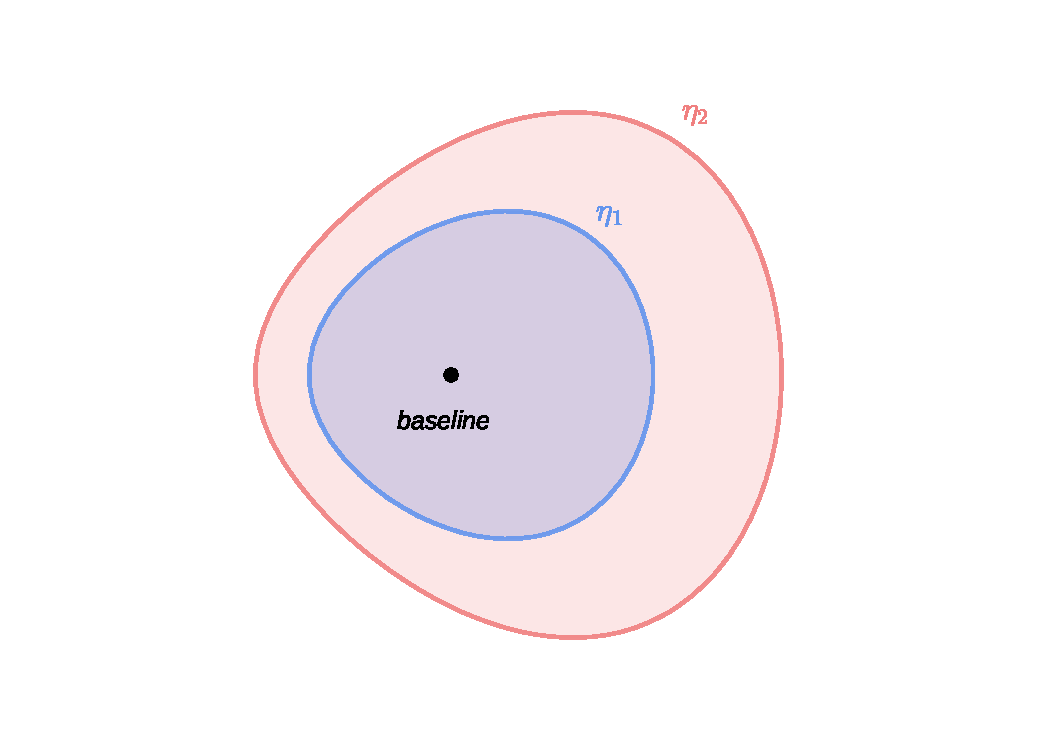
\includegraphics[width=1\textwidth]{eggs_backus.pdf}
\end{figure}
\end{frame}


\begin{frame}{Outcome of Hansen model}
Worst case mean distortion is a constant vector:

\begin{itemize} 
\item $$ w_t = \bar w  $$
\item Consequence is that contribution of $w_t$ to risk-prices is state-independent
\item Doesn't help explain countercyclical prices of risk (or prices of model uncertainty)
\end{itemize}
\end{frame}


\begin{frame}{Hansen and Sz\H{o}ke's more refined  dubious agent}

\begin{itemize}
\item Shares the econometrician's model $A, C, D, G$
\item Expresses doubts by using (a continuum of) likelihood ratios to form a discounted entropy ball around econometrician's model
\item Also insists that some  martingales representing  particular alternative {\em parametric} models be included in  discounted entropy ball .
\item Inclusion of those  alternative parametric models tilts the entropy ball  
\item That affects the worst-case model that attains a bound on values over this set of models in a way that can lead to countercyclical
uncertainty prices

\end{itemize}

\end{frame}


\begin{frame}[fragile]
  \frametitle{Concern about other parametric models}

Investor wants  to include particular alternative models with
\begin{align*}
E_t \left[\bar m_{t+1}\log \bar m_{t+1} \right]= \frac{1}{2}\bar w'_t \bar w_t = \xi(x_t)
\end{align*} and
discounted entropy
\begin{align*}
E^{\bar w}\left[ \sum_{t=0}^{\infty} \beta^t \xi(x_t)  \mid x_0, c_0 \right]
\end{align*}


{\textcolor{red}{How can this be done? }} 

By replacing earlier entropy constraint with
\begin{align*}
\frac{1}{2}E^{w}\left[ \sum_{t=0}^{\infty} \beta^t w'_t w_t  \mid x_0, c_0 \right] \leq E^{w}\left[ \sum_{t=0}^{\infty} \beta^t \xi(x_t)  \mid x_0, c_0 \right]
\end{align*} 
\end{frame}


\begin{frame}[fragile]
\frametitle{Yaron's bazooka}

Bansal and Yaron (2004) mix LRR with EZ preferences \\


\begin{itemize}
\item LRR is statistically difficult to detect and  estimate; but $\ldots$
\item Epstein-Zin or dubious agent really hates LRR
\begin{itemize}
\item \small{There are conditions under which EZ value function is  indirect utility function of dubious  agent}
\end{itemize}
\item That sets  stage for big risk-prices (but not countercyclical ones)
\end{itemize}

\end{frame}


\begin{frame}[fragile]
  \frametitle{Concern about bigger ``long-run risk'' in Sz\H{o}ke model}

Inspired by Bansal and Yaron (2004), an agent fears  particular long-run risks expressed by
\begin{align*}
x_{t+1} = \bar{A}x_t + C\widetilde \varepsilon_{t+1}
\end{align*}

\begin{itemize}
\item Corresponds to $\bar w_t = \bar w x_t$ with
\begin{align*}
\bar w = - C^{-1}(\bar A - A)
\end{align*}
\item Implies quadratic $\xi$ function:
\begin{align*}
\xi(x_t) := x'_t \bar{w}'\bar{w} x_t =: x'_t \Xi x_t
\end{align*}
\end{itemize}
\end{frame}



\begin{frame}[fragile]
  \frametitle{Tilted discounted entropy balls}
\begin{figure}
\includegraphics[width=1\textwidth]{eggs_backus2b.pdf}
\end{figure}
\end{frame}


\begin{frame}{State-dependent contributions to entropy constraint}

Time $t$ contributions to RHS of

\begin{align*}
\frac{1}{2}E^{w}\left[ \sum_{t=0}^{\infty} \beta^t w'_t w_t  \mid x_0, c_0 \right] \leq E^{w}\left[ \sum_{t=0}^{\infty} \beta^t \xi(x_t)  \mid x_0, c_0 \right]
\end{align*}

relax the discounted entropy constraint in states $x_t$ in which $\xi(x_t) $ is larger
  \quad \\
  \quad \\

This sets the stage for state-dependent mean distortions in worst-case model
\quad \\
\quad \\

These ignite countercyclical market prices of  uncertainty
\end{frame}

\begin{frame}[fragile]
	\frametitle{Sz\H{o}ke agent's sequence problem}

Linear quadratic problem
\small{
\begin{align*}
 J(x_0, c_0 \mid \Xi) &:= \max_{\tilde\theta\geq 0} \min_{\left\{w_{t}\right\}_{t\geq 1}} \ E^{w}\left[ \sum_{t=0}^{\infty} \beta^t c_t  + \tilde{\theta}\frac{1}{2}\sum_{t=0}^{\infty}\beta^t\left( w'_tw_t - x'_t\Xi x_t \right) \mid x_0, c_0 \right] \\
&  \text{s.t. } \ c_{t+1} - c_t = Dx_t + G ( \tilde\varepsilon_{t+1} - \textcolor{orange}{w_t} ), \quad\quad \textcolor{gray}{\tilde\varepsilon_{t+1}\sim \mathcal N(0, I)} \\
&\hspace{14.6mm} x_{t+1} = Ax_t + C( \tilde\varepsilon_{t+1} - \textcolor{orange}{w_t} )  % \\
%& \frac{1}{2}E^{w}\left[ \sum_{t=0}^{\infty} \beta^t w'_t w_t  \mid x_0, c_0 \right] \leq E^{w}\left[ \sum_{t=0}^{\infty} \beta^t \xi(x_t)  \mid x_0, c_0 \right]
\end{align*}}

Worst-case shock mean distortion
\begin{align*}
\widetilde{w}_t = \widetilde{w} x_t
\end{align*}

Worst-case model is $(\widetilde A, C, \widetilde D, G)$
\begin{align*}
\widetilde{A} & = A - C\widetilde{w} \\
\widetilde{D} & = D - G\widetilde{w} \\
\end{align*}
\end{frame}



\begin{frame}[fragile]
  \frametitle{Econometrician's model}
\begin{figure}
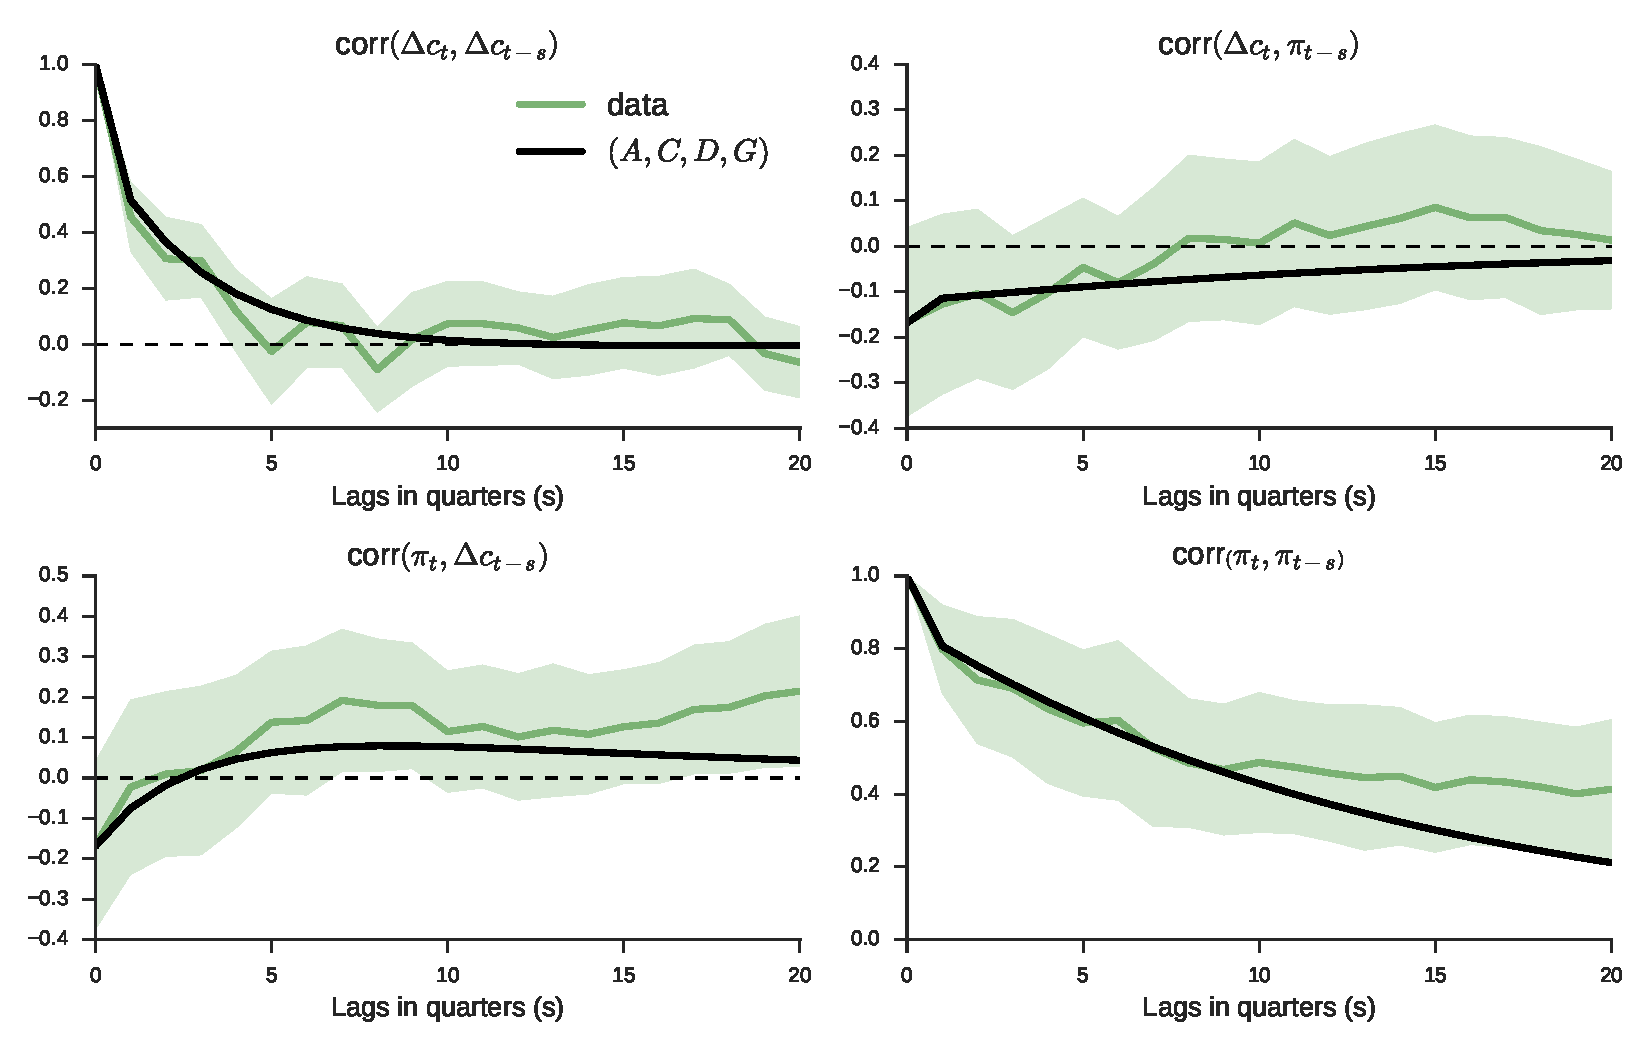
\includegraphics[width=\linewidth,height=\textheight,keepaspectratio]{fig2_tom.pdf}
\end{figure}
\end{frame}



\begin{frame}[fragile]
  \frametitle{US Term structure}
\begin{figure}
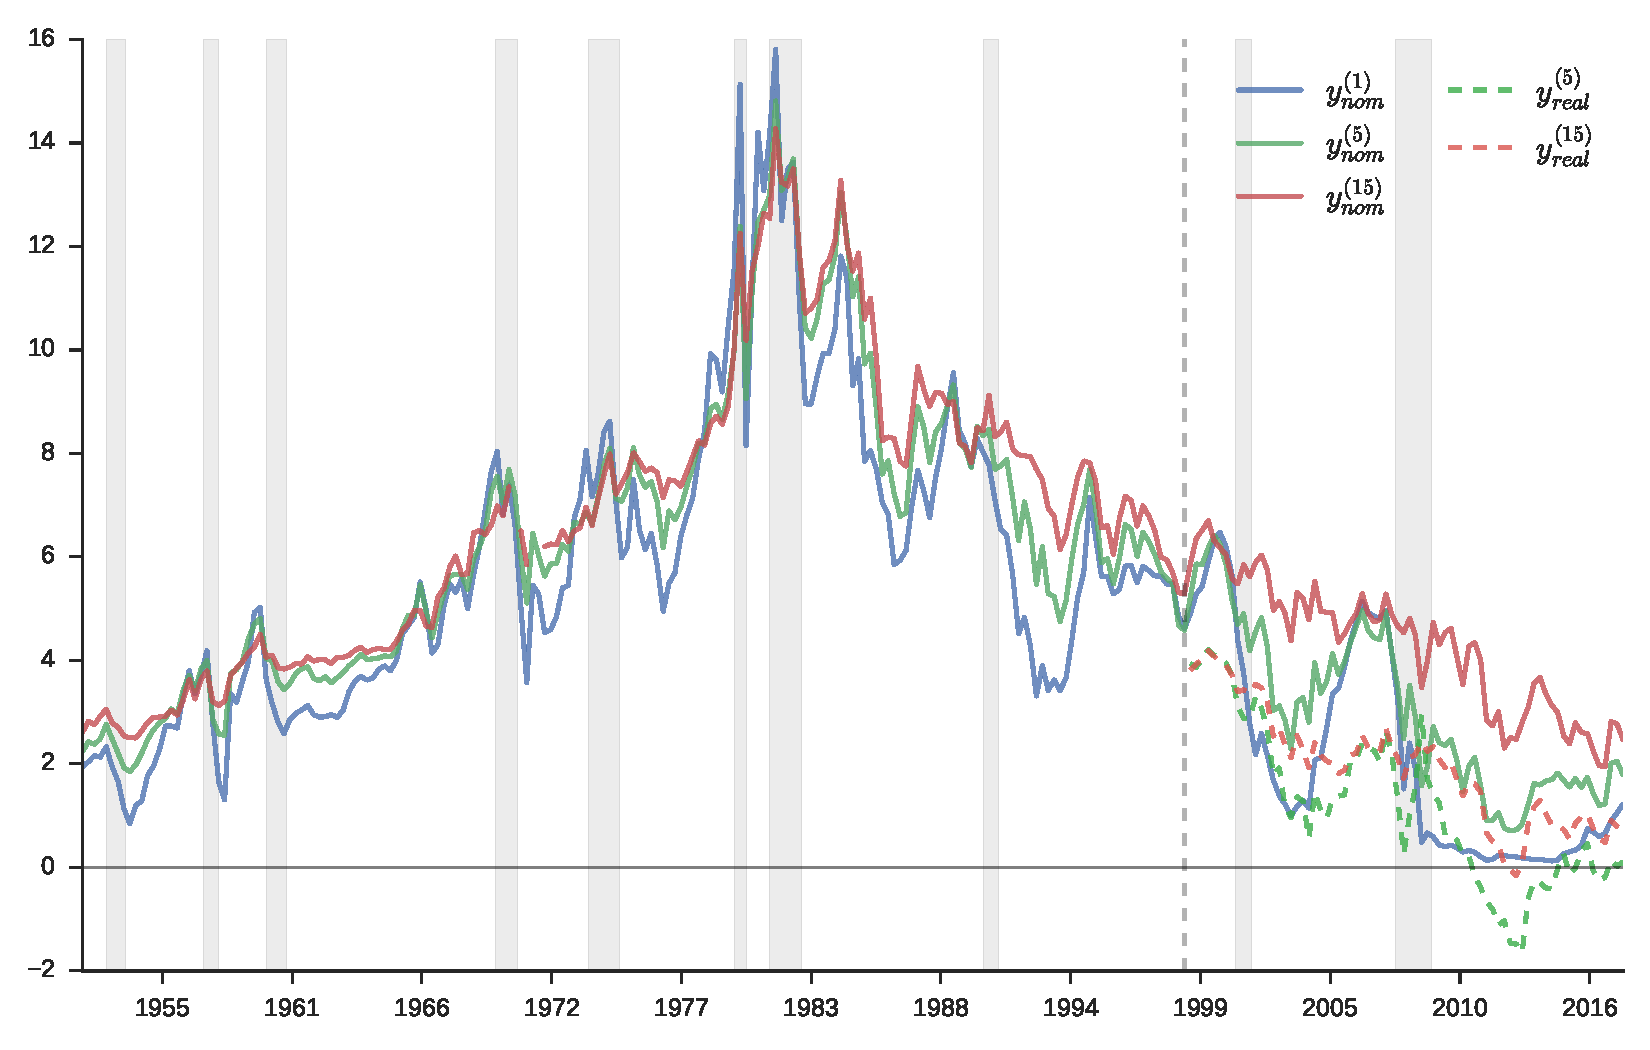
\includegraphics[width=\linewidth,height=\textheight,keepaspectratio]{fig1_tom.pdf}
\end{figure}
\end{frame}



\begin{frame}{Recognized patterns}

\begin{itemize}
 \item Nominal yield curve  usually slopes upward
 \item Long minus short yield spread narrows before US recessions,  widens after
 \item Consequently,  slope of yield curve helps predict  aggregate inputs and outputs
\item Long and short yields  are (almost) equally volatile (``Shiller puzzle'')
\item To solve ``Shiller puzzle'':  risk prices (or something observationally equivalent) must  depend on  volatile state variables
\end{itemize}

\end{frame}

%
%\begin{frame}{Possible table?}
%
%Might it be possible to make a table like this that accurately summarized flavor of results \textcolor{red}{Yes, it seems possible. I like this table}
%
%\begin{table}
%\begin{center}
%\begin{tabular}{lll}
%Average slope  & Slope near recessions & Describes \\ %$m_{t+1}$ \\
%\hline\\
%Lucas  &  no & no \\
%         &  &   \\
%Epstein-Zin  & no &   no   \\
%         & &   \\
%Hansen-Sargent (2001) & no & no \\
%  & & \\
%PSS &  yes   & maybe  \\
%         & &   \\
%Sz\H{o}ke & yes  & ``yes''  \\
%          & & \\
%%\hline \\
%\end{tabular}
%\caption*{Challenges and performances}
%\end{center}
%\end{table}
%
%\end{frame}


\begin{frame}{Challenges and responses}


\begin{table}
\begin{center}
\begin{tabular}{lccc}
& Average   & Slopes near  & Volatile\\
& slope    & recessions & long yield \\
\hline\\
Lucas (1978)  &  no & no & no \\
         &  &   \\
Epstein-Zin with LRR & maybe &   yes  &  no \\
(PS (2007), HS (2001))     & &  &  \\
&  &  & \\
%Hansen-Sargent (2001) & maybe & yes & no \\
%  & & & \\
PSS (2015) &  built-in  &  built-in & yes \\
         & & &  \\
Sz\H{o}ke (2017) & YES  & yes & yes \\
          & & & \\
%\hline \\
\end{tabular}
%\caption*{Challenges and performances}
\end{center}
\end{table}

\end{frame}

\begin{frame}{Forces at play}
\begin{itemize}
\item Affine risk prices with persistent consumption \emph{growth} can nail the 2nd column
\item 3rd column requires state-dependent  prices of risk
\end{itemize}



\end{frame}
%
%\begin{frame}{Possible table 2?}
%
%Might it be possible to make a table like this that accurately summarizes reason for the  results -- this
%draft is not correct at important points! \textcolor{red}{I'll think about this}
%
%\begin{table}
%\begin{center}
%\begin{tabular}{lll}
%Average slope  & Slope near recessions & Describes \\ %$m_{t+1}$ \\
%\hline\\
%Lucas  &  no & no \\
%         &  &   \\
%Epstein-Zin  & no &   no   \\
%         & &   \\
%PSS &  pessimism about XXXXX  & pessimism about XXXXX  \\
%         & &   \\
%Sz\H{o}ke & XXXXX  & long run risk concern  \\
%          & & \\
%%\hline \\
%\end{tabular}
%\caption*{Causes}
%\end{center}
%\end{table}
%
%
%\end{frame}



\begin{frame}{Three probability twisters }

\begin{itemize}
\item $w^*_t \sim $ Piazzesi, Salomao, Schneider's mistaken agent
\item $\bar w_t \sim $ Sz\H{o}ke's especial LRR parametric worry
\item $\tilde w_t \sim $ Sz\H{o}ke's worst-case model
\end{itemize}

\end{frame}

\begin{frame}{Motivation}
 \begin{quote}
  An appealing feature of robust control theory is that it lets us deviate from
  rational expectations, but still  preserves a set of powerful cross-equation restrictions on  decision makers'
  beliefs $\ldots$ %provided that an {\em ex post} Bayesian interpretation is applicable.
    Consequently,
  estimation  can proceed essentially as with
  rational expectations econometrics.  The main difference is that now  restrictions through which we
  interpret the data emanate from the decision maker's best response to a  worst-case model instead of to the
  econometrician's model. \quad Sz\H{o}ke (2017)
 \end{quote}



\end{frame}



\begin{frame}{Sz\H{o}ke's empirical strategy, I}
\begin{itemize}
\item Use $\{x_t, c_t\}_{t=0}^T$ to estimate the econometrician's $A, C, D, G$
\item View $\Xi$ as matrix of additional free parameters and estimate them simultaneously with  risk prices  $\tilde \lambda x_t$
in $\tilde \lambda_t = \tilde \lambda x_t$ from  data $\{p_t(n+1)\}_{n=1}^N, t=0, \ldots, T$ by imposing  cross-equation restrictions
\begin{align*}
p_t(n+1) = & \exp(- r_t) E_t \left[ m_{t+1}^{\tilde w} m_{t+1}^{\tilde \lambda}   p_{t+1}(n) \right] \\
%\end{align*}
% where discounted entropies of all models are constrained to be inside
%a $\bar w_t$-twisted entropy ball.
%\begin{align*}
m_{t+1}^{\tilde w}  = & \exp \left(
- \tilde w_t' \varepsilon_{t+1} - \frac{\tilde w_t'
\tilde w_t}{2} \right)  \cr
m_{t+1}^{\tilde \lambda}  = & \exp\left(- \tilde \lambda_t \varepsilon_{t+1} - \frac{\tilde \lambda_t' \tilde \lambda_t}{2} \right)
\end{align*}

where $E_t$ is taken with respect to the econometrician's  model and
 $ \tilde w_t = \tilde  w x_t$ is the dubious investor's worst-case model.
\end{itemize}
\end{frame}



\begin{frame}{Sz\H{o}ke's empirical strategy, II}
\begin{itemize}
\item Assess improvements in predicted behavior of term structure of interest rates
\item Use estimated worst-case dynamics to form distorted forecasts $\tilde  x_{t+1} = (A - C \tilde w) x_t$ and compare them
to those of professional forecasters.
\item Compute discounted relative entropy of worst-case twisted model $(A - C \tilde  w), C, (D - G \bar w), G$ relative to the econometrician's model
$A, C, D, G$ and use it and Chernoff-Newman-Stuck entropy measures to assess difficulty of distinguishing  two models.
\end{itemize}

\end{frame}



\begin{frame}{Interpretations from Sz\H{o}ke  model}
Conditional mean distortions $w x_t$:
\begin{itemize}
\item PSS: $ w^*_t$ is vector of ``mistakes'' or ``suboptimal forecasts''
\item Sz\H{o}ke: $\tilde  w_t$ is vector of ``model uncertainty'' prices:  compensations that Sz\H{o}ke's representative
agent charges to bear risks   $\varepsilon_{t+1}$  with unknown probability distribution
\end{itemize}

\end{frame}


\begin{frame}{Insights from Sz\H{o}ke's  model}
\begin{itemize}
\item A theory of state-dependent belief distortions $\tilde w_t = \tilde w x_t$
\item A theory about the question that professional forecasters answer:
\begin{itemize}
\item they  answer with their
worst-case model because they hear  ``tell me forecasts that rationalize your (max-min) decisions''
\end{itemize}
\item A way to measure size of  belief distortions  relative to the  econometrician's model
\end{itemize}

\end{frame}




\begin{frame}{Insights from Sz\H{o}ke's  model, II}

He uses his  estimated $\Xi$ matrix

\begin{itemize}
\item To infer an equivalence class of alternative parametric models parameterized by $\bar w$ that concerns the representative investor
 \begin{itemize}
 \item  \small{Models have  more long-run risk than econometrician's model }
 \end{itemize}
\item To infer a  worst-case mean distortion $\tilde w x_t$ whose state dependence causes the term structure to move with $x_t$ in ways that  explain hitherto puzzling term structure movements (e.g., Shiller's ``volatility puzzle'')
\end{itemize}

\end{frame}

\begin{frame}{Who cares?}
Joint probability distributions of interest rates and  macroeconomic shocks  are important in macroeconomics
\begin{itemize}
 \item Costs of aggregate fluctuations (business cycles)
 \item Consumption Euler equations (aka `New Keynesian IS curves')
 \item Optimal taxation and government  debt management
 \item Central bank `expectations management' strategies
 \item Long-run risk (aka `secular stagnation')
\end{itemize}

\end{frame}
%
%\begin{frame}{David Backus}
%
%
%Dave Backus contributed immensely and graciously to what we know   and how we can go about learning more
%
%\medskip
%
%\medskip
%
%Rather than curse  darkness, Dave  lit candles
%
%\end{frame}

\end{document}


\begin{frame}{Backup slides}

\end{frame}





\begin{frame}[fragile]
	\frametitle{Bellman-Isaacs}

\end{frame}



\begin{frame}[fragile]
  \frametitle{Multiplier problem}

Multiplier preference version
\begin{align*}
 W(x_0, c_0 \mid \theta) := \min_{\{m_{t+1}\}_{t\geq 0}} \ & E\left[ \sum_{t=0}^{\infty} \beta^t \textcolor{orange}{M_t} \left(c_t + \theta m_{t+1}\log m_{t+1} \right) \mid x_0, c_0 \right] \\
  M_{t+1} &= M_tm_{t+1}, \quad E[m_{t+1} \mid x_t, c_t] = 1, \quad M_0 = 1
\end{align*}

Recursive formulation
\begin{align*}
 W(x_t, c_t \mid \theta) &= c_t + \min_{m_{t+1}} \ E\left[ m_{t+1}\left[\beta W(x_{t+1}, c_{t+1}) + \theta\log m_{t+1} \right] \mid x_t, c_t\right] \\
 &= c_t - \theta\log E\left[ \exp\left( - \frac{\beta W(x_{t+1}, c_{t+1})}{\theta}\right) \mid x_t, c_t \right] \\
 &:= c_t + T_t\left[\beta W(x_{t+1}, c_{t+1})\right]
\end{align*}
RHS attained by
\begin{align*}
m^*_{t+1} \propto \exp\left( - \frac{W(x_{t+1}, c_{t+1})}{\theta}\right)
\end{align*}


\end{frame}


\begin{frame}{Relationship between multiplier and constraint problems}

Application of Lagrange multiplier theory:

$$ W(x_t, c_t \mid \tilde \theta) = J(x_t, c_t \mid \eta) + \tilde \theta \eta $$


\end{frame}


\begin{frame}{Stochastic discount factor }

%Encoding   risk aversion as belief distortion


%Stochastic discount factor:

\[  \]

\begin{itemize}
\item $s_{t+1} = \exp(- r_t ) m_{t+1}  $
\item $\exp(-r_t)$ discounts for one period ahead
\item $m_{t+1}$ discounts for covariance of payouts with felicities
\end{itemize}


\end{frame}


\begin{frame}{ $ s_{t+1} = \exp(- r_t ) \exp(-\lambda_t \varepsilon_{t+1} - \frac{1}{2} \lambda_t' \lambda_t)   $}



\begin{itemize}
%\item $ s_{t+1} = \exp(- r_t ) \exp(-\lambda_t \varepsilon_{t+1} - \frac{1}{2} \lambda_t' \lambda_t)   $
\item $\exp(-r_t) \sim$ discounts one-period risk-free payouts
\item $\lambda_t \sim $ increase in expected return earned for bearing   exposure to $\varepsilon_{t+1}$-risk
\item $\lambda_t \sim$ ``price of risk'' vector
\end{itemize}

\end{frame}

\end{document}
%
